\documentclass[dvisvgm,tikz,margin=2pt]{standalone}
\usepackage{amsmath,amssymb,amsthm,mathtools}
\usepackage{tikz}
\usetikzlibrary{positioning,calc}
\usepackage{xcolor}
\newcommand{\R}{\mathbb{R}}
\newcommand{\Q}{\mathbb{Q}}
\newcommand{\abs}[1]{\lvert #1\rvert}
\newcommand{\norm}[1]{\lVert #1\rVert}
\newcommand{\RSSP}{\textsc{Riesz-Subset}}
\newcommand{\MIS}{\textsc{Independent-Set}}
\newcommand{\sgnspin}{\{-1,+1\}}
\begin{document}
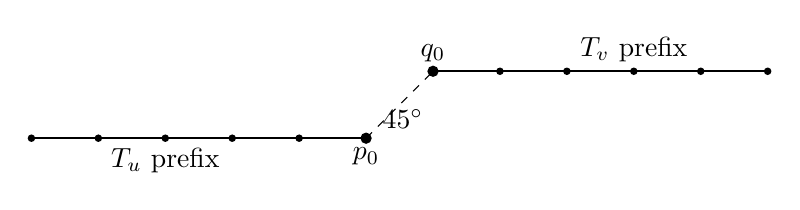
\begin{tikzpicture}[scale=0.85]
  \draw[thick] (-5,0)--(0,0);
  \draw[thick] (1,1)--(6,1);
  \fill (0,0) circle (2.4pt) node[below] {$p_0$};
  \fill (1,1) circle (2.4pt) node[above] {$q_0$};
  \foreach \x in {-1,-2,-3,-4,-5} \fill (\x,0) circle (1.6pt);
  \foreach \x in {2,3,4,5,6} \fill (\x,1) circle (1.6pt);
  \draw[dashed] (0,0)--(1,1);
  \node at (0.55,0.28) {$45^\circ$};
  \node[below] at (-3,0) {$T_u$ prefix};
  \node[above] at (4,1) {$T_v$ prefix};
\end{tikzpicture}
\end{document}
